\chapter{Basics}
\textcolor{red}{
Everything necessary to understand the implementation as well as anything which is done beforehand, will come up here}

In the following, all concepts, technologies and required backgrounds for understanding this thesis are explained. Firstly data and data types are described. Secondly diagrams and how they are structured are described. Lastly D3 as a tool to create diagrams is described.


\section{Data}
\textcolor{red}{
Well talk about data a bit. Where does it come from? How is it structured? What kind of attributes? What even are attributes?}

Since ancient times, humans have recorded data. Recording the ins and outs of available resources was one of the driving factors behind the conceptualization of writing. (TODO: Check sources of the beer brewing video series)
With the introduction of computers the amounts of gathered data have grown drastically. Nowadays vast amounts of data are gathered across all aspects of life.

\begin{figure}
    \label{fig:data-visualization}
    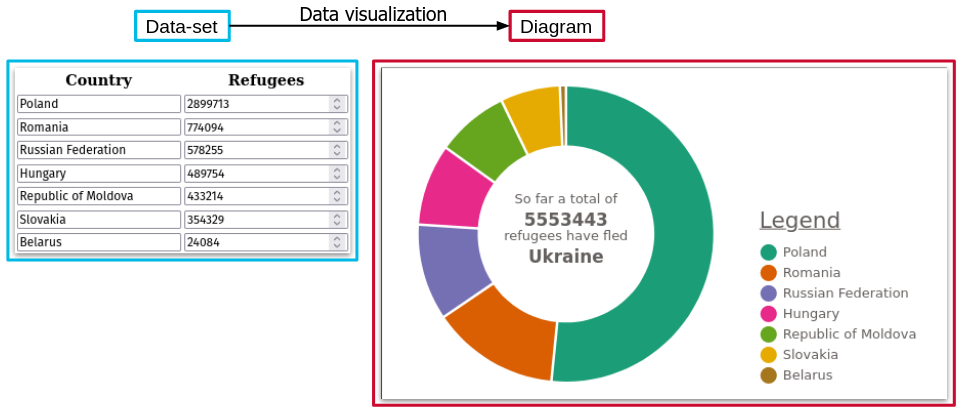
\includegraphics[width=\linewidth]{data-visualization2.png}
    \caption[data-visualization]{Where data visualization comes into play.}
\end{figure}

The vast amounts of data gathered in databases are often hard to comprehend and evaluate with the human mind. They are also unwieldy to present them in the often limited space of articles, dashboards or other informative purposes. Therefore data visualization (Figure \ref{fig:data-visualization}) is used to turn these datasets, collections of data-points, into diagrams.

Data is commonly preprocessed before turning it into diagrams. Depending on the dataset and the desired result, this can mean different things. One might want to remove excessive information from the dataset, which is not necessary for the representation. On the other hand, additional data can be added by evaluating the existing data-points. These could for example be the median of values or grouping of certain value ranges. It is important to note, that this preprocessing can happen with specific intentions in mind. While it is only supposed to make the representations easier and more concrete, it can be abused to make data align with the desired results or to create a certain emphasis. This thesis is not too concerned with this, as the possibilities of D3 have nothing to do with the correctness of the chosen data.

Even though data comes from a huge variety of sources and can express a plethora of things, there are only four different types of data. They are split into two categories. Categorical and numerical data. Each category has two subtypes. In the following each of the types of data will be explained.

\subsection{Categorical}
\textcolor{red}{
What is categorical data? Nominal and ordinal data}

Categorical or qualitative data is information collected in groups. It is often of descriptive nature. Whilst the values can be represented in numbers, they do not allow for arithmetic operations.
There are two types of categorical data. Nominal and ordinal data.

\paragraph{Nominal}
data is mostly descriptive in nature. They are independent and have no inherited order. Examples are 'Country of origin', 'Color of paint', 'Brand of car'.

\paragraph{Ordinal}
data is also descriptive, yet the data does have a internal order. For example different dates each describe a day, but one day also comes after another. Grades also have an internal order, as one grade is better then another. Whilst ordinal data has an ordering, the order is not necessarily equidistant.

\subsection{Numeric}
\textcolor{red}{
What is numeric data? Continuous and Discrete}

Numeric or quantitative data is all data expressed in numbers, where numbers do not represent categories. It allows for arithmetical operations and can be split into discrete and continuous data.

\paragraph{Discrete}
data can only take certain defined values. This usually means whole numbers to represent things that can not be split up further. Like the 'Number of Refugees' or 'Tickets sold'. Discrete data is countable.

\paragraph{Continuous}
data can be measured. It can have any real number as value. Therefore fractions are possible as well. For example when measuring the temperature, or the length or weight of an object.


\section{Diagrams}
\textcolor{red}{
What diagrams exists? Which are the most common? What possibilities do they offer for encoding data? Which considerations for readability? Why do some diagrams not make as much sense? Which considerations where made for fulfilling the showcase requirements?}

We constantly come across the results of data visualization in everyday life. They can be commonly found across all kinds of reports, information campaigns or as part of user-interfaces in machinery or control systems. Yet the selection of which diagram should be used to visualize which data-set is not trivial. Mostly there are several possible diagram choices for the given data. Furthermore there are a plethora of diagrams already in use and anyone can create totally new diagrams to suit their needs. Yet there are diagrams which are used more commonly. These include bar and pie-charts, scatter plots and heat-maps (TODO: Find source (lel)).

Whilst there are countless types of diagrams, all diagrams use a combination of marks and channels to encode data. Marks are used for entries in the diagram. Channels describe the way specific marks encode data. The three possible marks are points, lines and areas. Each mark should use at least one channel to encode data. Otherwise it does not convey any information. The most commonly used channels are position, size, color and texture. The position in 2D can be split into the x and y positions. The color is split into hue and luminescence. For example looking at fig. \ref{fig:bar-chart} we can see lines being used as marks for each entry. It might seem like we are using areas, but the thickness of the line only serves visual understanding. The lines also use three channels to encode data. The y-position is used to represent the categorical data of which country. The hue of the bar encodes the same data. This is a big redundant, as the country is already encoded. Yet the hue makes it easy to follow along when data is changing and bars are shifting positions. The size, in this case length, of the bar encodes the discrete data of how many refugees have crossed into the country. In fig. \ref{fig:donut-chart} we see areas used as marks. Just like in the previous example the hue encodes the country and the size encodes the refugee count. 

All marks can be used with all channels. But not all data types should be represented by all channels. For example nominal data should not be encoded using the size channel. The different sizes would lead to a perceived order, which does not exist in nominal data. As the channels all differ in their appearance they are also not equally good in adequately representing the data types. Therefore it is important to consider which channels are chosen to represent the given data types. Therefore the selection of marks and channels should be considered carefully. If chosen poorly it can lead to undermine the purpose of the diagram, easily presenting data to a viewer. According to a study by Jock Mackinlay from 1986, the position channels can always be considered the strongest channels, no matter which marks are combined with it\cite{mackinlay1986automating}.


\begin{figure}
    \label{fig:bar-chart}
    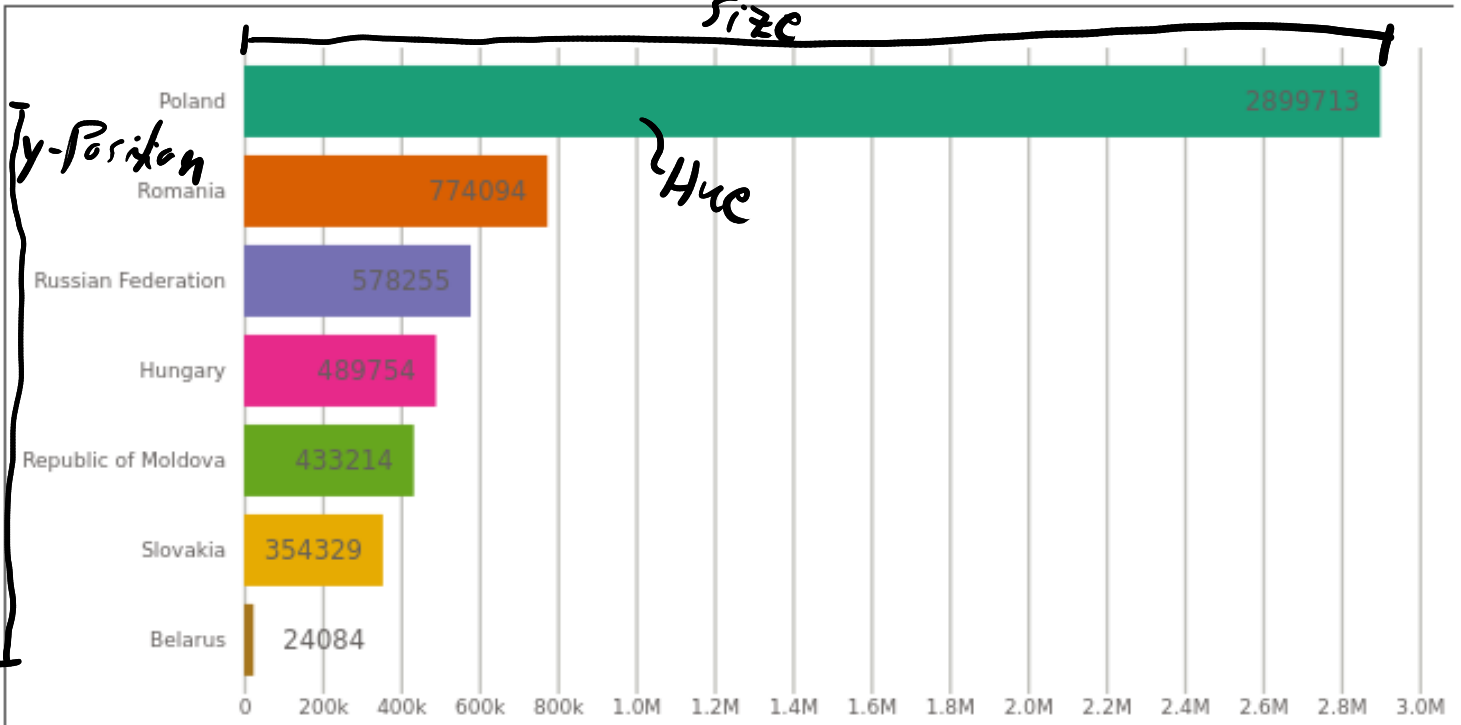
\includegraphics[width=\linewidth]{bar-chart-channels.png}
    \caption[bar-chart]{This is a bar-chart with used channels shown.(TODO: which needs a frame..? Also draw in marks and channels)}
\end{figure}

\begin{figure}
    \label{fig:donut-chart}
    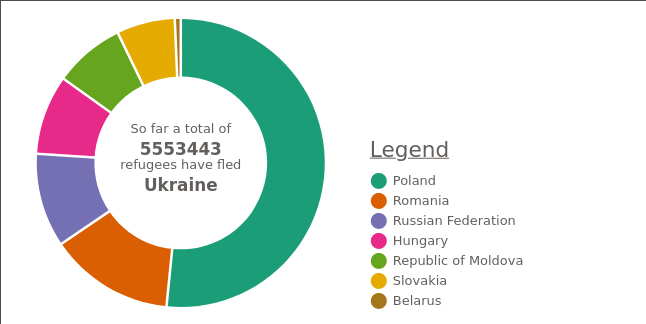
\includegraphics[width=\linewidth]{donut-chart.png}
    \caption[donut-chart]{This is a donut-chart (TODO: which needs a frame..? Also draw in marks and channels)}
\end{figure}

\section{D3.js}
This is all about d3. What is it? Where does it come from? What is it used for? Who uses it? Why should it be used? How does it work? Enter, update and exit pattern. Something about the modular structure of D3 as well. Might be worth mentioning "observables" as well.

"D3.js is a JavaScript library for manipulating documents based on data. D3 helps you bring data to life using HTML, SVG, and CSS."\cite{d3js}. The name D3 is short for data-driven documents. The D3 library was originally created by Mike Bostock and is published under the BSD-3-Clause open-source license. It is about 500kb in size. It does not require a specific framework and can therefore be easily integrated into all kinds of web based projects. Whilst D3 is not limited to using svg, the visualization created using D3 mostly rely on svg elements for their implementation.

D3 is not a high-level API for creating out of the box visualizations. Instead it is a library which aims at making the tedious parts of DOM manipulation easier. It also provides some helper functions, scales, to decrease the amount of mathematical equations needed to convert from the data extends to the necessary coordinates in the desired visualization.

TODO: merge the section above and below to one longer introduction

General functioning of D3.

"D3 allows you to bind arbitrary data to a Document Object Model (DOM), and then apply data-driven transformations to the document."\cite{d3js}. There are three main concepts that make up the core of D3. Selections, data joins and the general update pattern. All three of these concepts are working closely together. Whilst selections can be used without data joins and the general update pattern, these two aspects both rely on selections. Data joins can also be used without explicitly using the general update pattern. Usually all three of these concepts are used consecutively. First a selection is created. This selection is provided with a data join. Finally the behaviors for the general update pattern are defined for this data join.
In the following all three of the core concepts of D3, as well as scales and D3's modularity are explained.

\subsection{Selections}
\textcolor{red}{
What are they? Why are they useful?}

All operations in D3 run on an arbitrary collection of nodes. These collections of nodes are called selections. There are two functions in D3 to create a new selection: \verb|d3.select("selector")| and \verb|d3.selectAll("selector")|. Both functions require a selector for identifying the appropriate elements. The selectors are defined in the W3C Selectors API\cite{w3c_selectors_api} and function like CSS selectors. Whilst select only selects a single element, the first element matching the selector, selectAll selects all elements which match the selector. It is important to note, that select also propagates the existing information of this node, whilst selectAll does not.
Selections can also be extended or shrunken by adding or removing nodes, or by combining multiple selections.
It is possible to directly access DOM elements through the selections. The respective DOM elements are linked in the nodes which make up the selection. But usually this is not required, as there are predefined functions for modifying the nodes properties. This includes the modification of attributes and styles, as well as event handling. 

\subsection{Data Joins}
\textcolor{red}{
What are they and why are they important?}

Data joins are a key feature of D3. They link up a specific data-point to a specific DOM element. To create a data-join, one has to call the \verb|.data(dataset)| function on a selection. It takes a dataset, an array of data-points, as parameter. This will bind the data-points to the nodes in the selection. This is achieved by using an identifier function. The default identifier function returns the index of the data-point in the dataset. When we want to create diagrams which can respond to data changes over time, this is not a reliable identification. When data-points are removed or added in arbitrary locations, the index will not match the elements it previously did. Therefore we can specific a custom identifier function. This is passed as the second parameter of the data function, will be called for each data-point and has to return some value which will be used as an id.

When creating a data join, it can be that the number of data-points does not match up with the number of elements to represent them. Therefore the data-joins provide an empty placeholder node to all data-points which are not matched up with an element. What happens to the placeholders is defined in the general update pattern.

\subsection{General Update Pattern}
\textcolor{red}{
What is it? What can it do? Describe data joins and dom element links.}

\begin{figure}
    \label{fig:general-update-pattern}
    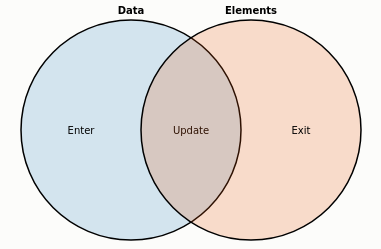
\includegraphics[width=\linewidth]{general-update-pattern.png}
    \caption[general-update-pattern]{A visual representation of the make up of the general update pattern\cite{bostock_2012}}
\end{figure}

The general update pattern is another core concept of D3. Every time a data join is created or updated, it comes into play. The general update pattern differentiates between three different cases. For each of these cases a sub-selection is created. For each of these three selections the behavior can be defined. The first selection is the enter selection. All data-points which have been matched up with a placeholder node while creating the data-join are in here. In the behavior for the enter selection, usually a corresponding element is created as the first step.

All the elements which are already linked to a data-point using the identifier function, make up the update selection. The last selection, the exit selection, is made up of all the elements for which the corresponding data-point has been removed. The behavior of the exit selection is by default defined to remove the respective elements.

When the goal is to create only static diagrams, which are only initially created from data, it is enough to define the behavior for the enter selection, as all data-points will be matched up with a placeholder when creating the data-join. Here the identifier function is also not important, as the created element will not need to change over time and therefore do not need to be able to be appropriately selected again as data changes. If diagrams should be able to react to data changes and update their appearance, like in this thesis, it is also important to define the update behavior as well as a proper identifier function, so elements are always matched with the same data-points. The exit behavior can be defined if a more visually pleasing removal of elements is desired, like fading out before deleting.


\subsection{Scales}
\textcolor{red}{
What are scales? What do they do? Why and when are they used? How do they look like?}

Scales are a way to convert between two data-spaces. Some scales can even convert between two data-types. Scales can be found in many places. For example converting percentages of correct answers in a test, continuous data, to the appropriate grade, ordinal data. Or the scale factor of maps and model-kits.

As most diagrams created with D3 are created as SVG, the scales provided by D3 are mostly used to convert from the data-space to the coordinate space in which elements should be drawn. All scales require a domain and a range. The domain describe the input values, the range where they should map to. Some types of scales also allow to be used in reverse. 

\subsection{Modules}
\textcolor{red}{
The way D3 is split up into modules, the core package and what kind of extensions are there.}

D3 provides the most used, general functionalities in the core library. Yet there are many more modules which can be added, which add functionalities for more specific use-cases.
